\documentclass[12pt, oneside]{article}
\usepackage[letterpaper, margin=1in, headsep=0.5in]{geometry}
\usepackage[english]{babel}
\usepackage[utf8]{inputenc}
\usepackage{amsmath}
\usepackage{amsfonts}
\usepackage{amssymb}
\usepackage{tikz}
\usetikzlibrary{quotes, angles}
\usepackage{graphicx}
%\usepackage{pgfplots}
%\pgfplotsset{width=10cm,compat=1.9}
%\usepgfplotslibrary{statistics}
%\usepackage{pgfplotstable}
%\usepackage{tkz-fct}
%\usepackage{venndiagram}

\usepackage{fancyhdr}
\pagestyle{fancy}
\fancyhf{}
\rhead{\thepage \\Name: \hspace{1.5in}.\\}
\lhead{BECA / Dr. Huson / Geometry 10th Grade\\* Learning trajectory: Area, perimeter, volume}

\renewcommand{\headrulewidth}{0pt}

\begin{document}
\subsubsection*{Area, perimeter, volume}
  \begin{enumerate}
  \item Rectangle, square area and perimeter
  \item Circle area and circumference
  \item Sector areas, arc length
  \item Solve for parameter versus calculate result
  \item Compound shapes (including margins)
  \item Distance on the coordinate plane
  \begin{enumerate}
    \item Plotting, labeling points, etc.
    \item Horizontal \& vertical distances
    \item Pythagorean formula
    \item Applications: Rhombus, isosceles $\triangle$,
    \item Radicals, $\pi$ and rounding
    \end{enumerate}
  \item Triangle area, perimeter (formula sheet)
  \item Volume: prism, cylinder, cone
  \item Surface area
  \item Scaling shapes (eg. rectangle, triangles including midline)
  \end{enumerate}

  \begin{enumerate}
    \subsubsection*{Basic shapes}
    \item Regents problems, January 2017, \#26, 34, 29?

\subsubsection*{Distance on the coordinate plane, proofs}
  \item Given the quadrilateral $RSTU$ with $R(1,3)$, $S(4,7)$, $T(4,2)$, and $U(1,-2)$.
    \begin{enumerate}
      \item Plot and label $RSTU$ on the grid.
      \item Using the distance formula or otherwise, calculate $RS$, $ST$, $TU$, and $RU$.
      \item Definition: If a quadrilateral has four congruent sides, then it is a rhombus.\\[0.5cm]
      Prove that $RSTU$ is a rhombus.
    \end{enumerate}
    \begin{center} %4 quadrant regents grid w T-Chart
    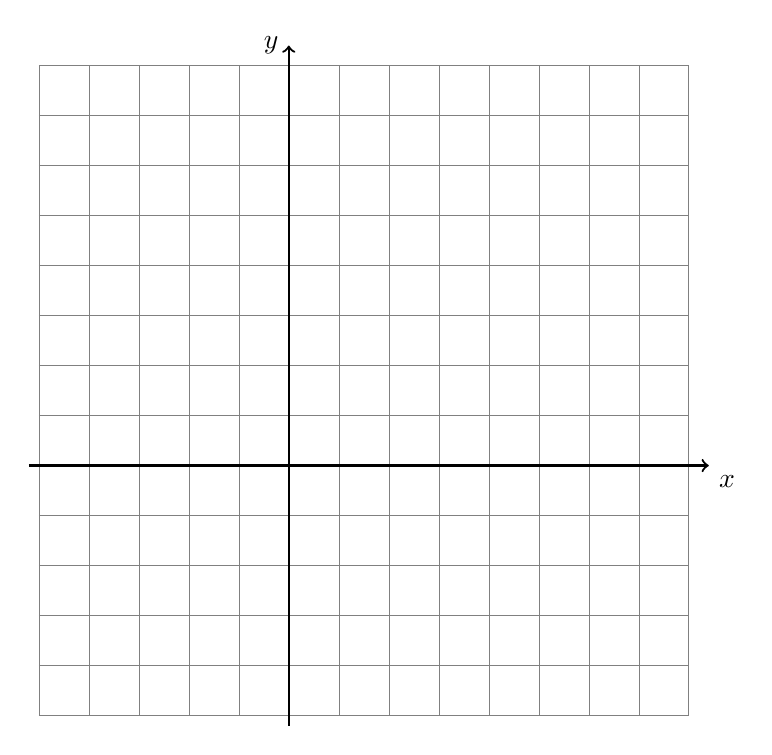
\begin{tikzpicture}[scale=.635]
      \draw [help lines] (-5,-5) grid (8,8);
      \draw [thick, ->] (-5.2,0) -- (8.4,0) node [below right] {$x$};
      \draw [thick, ->] (0,-5.2)--(0,8.4) node [left] {$y$};
    \end{tikzpicture}
    \end{center}

  \item Given the quadrilateral $RECT$ with $R(-4,1)$, $E(8,1)$, $C(8,6)$, and $T(-4,6)$.
    \begin{enumerate}
      \item Plot and label $RECT$ on the grid.
      \item Using the distance formula, calculate the length of the two diagonals $RC$ and $ET$.
      \item Theorem: If the diagonals of a quadrilateral are congruent, then it is a rectangle.\\[0.5cm]
      Prove that $RECT$ is a rectangle.
    \end{enumerate}
    \begin{center} %4 quadrant regents grid w T-Chart
    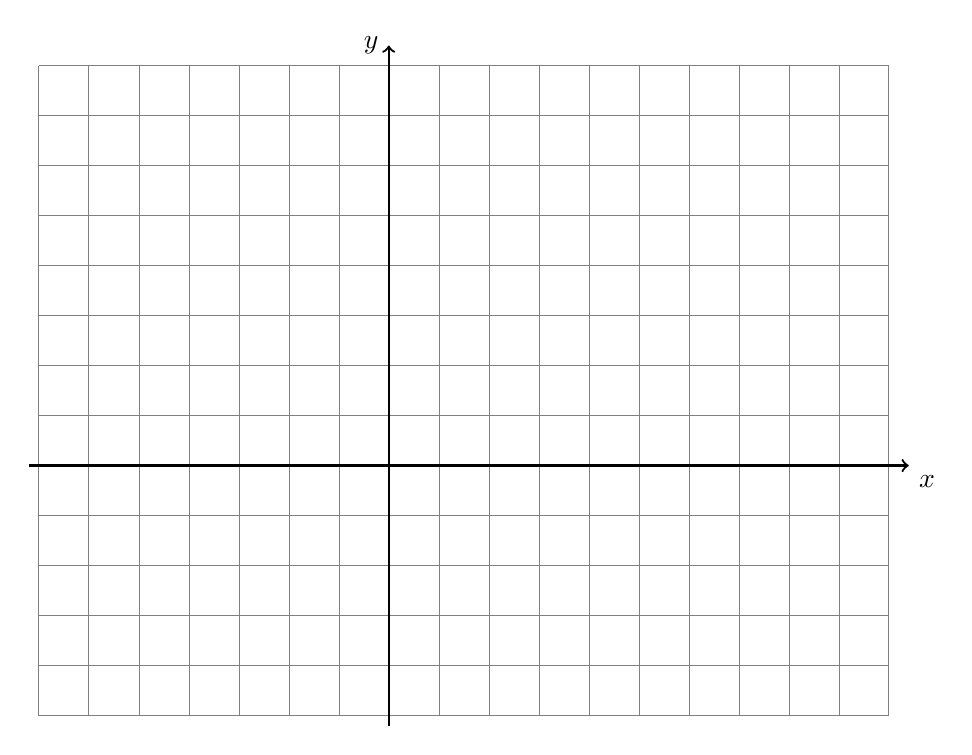
\begin{tikzpicture}[scale=.635]
      \draw [help lines] (-7,-5) grid (10,8);
      \draw [thick, ->] (-7.2,0) -- (10.4,0) node [below right] {$x$};
      \draw [thick, ->] (0,-5.2)--(0,8.4) node [left] {$y$};
    \end{tikzpicture}
    \end{center}

  \end{enumerate}

\end{document}
